\documentclass{article}
\usepackage[utf8]{inputenc}
\usepackage[nottoc]{tocbibind}
\usepackage{latexsym}
\usepackage{amsmath}
\usepackage{amsthm}
\usepackage{amsfonts}
\usepackage{amssymb}
\usepackage{tikz}
\usetikzlibrary{math}
\usepackage{bm}
\usepackage{booktabs}
\usepackage{adjustbox}
\usepackage{url}
\usepackage{cancel}
\usepackage{caption}
\usepackage{subcaption}
\usepackage{graphics}
\usepackage{algorithm}
\usepackage[noend]{algpseudocode}
\usepackage{float}
\usepackage[hidelinks]{hyperref}
\usepackage{listings}
\usepackage{mathtools}
\usepackage{epsfig}
\usepackage{wrapfig}
\usepackage{psfrag}
\usepackage{pgfgantt}
\usepackage{multirow}
\usepackage{comment}
\usepackage{arydshln}
\usepackage{float}

\newtheorem{definition}{definition}[section]
\newtheorem{hypothesis}{hypothesis}[section]
\newtheorem{theorem}{theorem}[section]
\newtheorem{prop}{proposition}[section]
\newtheorem{lemma}{lemma}[section]
\newtheorem{example}{example}[section]
\newtheorem{remark}{Remark}[section]

\title{
  % On Some Recently Developed Numerical Methods\\
  % for Nonuniform Fast Fourier Transform
  A Variety of Approaches to \\
  the Nonuniform Fast Fourier Transform
}

\author{
  Connor Robertson and Kosuke Sugita
}
\date{December 14, 2021}

\begin{document}

\maketitle


% TODO:
% - summarize the research area and approaches
%   use Townsend's summary

% \begin{itemize}
%   \item kernels (window functions)
% \end{itemize}

\section{Introduction}

There are many signal and image processing applications in which real or frequency space samples are collected non-uniformly.
As a result, analyzing the Fourier spectrum of nonuniform samples or evaluating points from non-uniform frequency data has been a focus of numerical analysts for more than half a century. % TODO: Citation?
Although this can be easily accomplished using the direct discrete Fourier transform (DFT) sum of non-uniform samples $(x_n, f(x_n))$ where $x_n = \frac{2\pi n}{N}$:
\begin{align*}
  \hat{f}(k) = \sum_{n=0}^{N-1} f(x_n) e^{-2i \pi k \frac{n}{N}}
,\end{align*}
this summation is of order $O(N^{2})$.

It would be preferable to reduce the computational burden of this process via the fast Fourier transform (FFT).
This algorithm can reduce the computational cost to $O(N\log{N})$ by taking advantage of the symmetry provided by uniform sampling:
\begin{align*}
  \hat{f}(k) = \sum_{n=0}^{\frac{N}{2}-1} f(x_{2n})e^{-2i \pi k \frac{2n}{N}} + e^{-2i\frac{\pi k}{N}} \sum_{n=0}^{\frac{N}{2}-1} f(x_{2n+1}e^{-2i \pi k \frac{2n}{N}})
.\end{align*}
Due to this symmetry requirement, it cannot be directly applied to non-uniform points.

Thus, there has been significant effort to accurately and cheaply remap the non-uniform samples to a uniform grid which can then be transformed via the FFT.
This has become known as the non-uniform fast Fourier transform (NUFFT) the key component of which is the procedure used to map the non-uniform samples to uniform samples.

Several approaches have been proposed for this initial mapping including polynomial or spline interpolation, delta spike smoothing via smooth kernel functions, and low rank representations of the DFT matrix. % TODO: Citation?
Many inroads have been made to maximize speed and accuracy with these methods, but the exact mapping procedure is still an active research topic.

In this report, we explore the variety of approaches for mapping non-uniform to uniform points including the most popular smoothing kernels and the low-rank approximation.
We complement this discussion with some programming exploration and examples using our own code as well as established NUFFT libraries.

\section{Numerical methods}


\subsection{Gaussian kernel NUFFT}
%TODO: fill a few pages on Type-3 NUFFT with Gaussian kernel here.

First,
Since Type-$1$ and Type-$2$ have been covered in the class, we avoid repeating the same discussions on these types.
Instead, here we describe Type-$3$ NUFFT with Gaussian kernel based on \cite{JCP-2003-Greengard}.
The main idea of Type-$3$ is to sandwich an intermediate uniform data between the input and output data both of which are nonuniform.
The procedure is summarized as follows.
\begin{enumerate}
  \item Split the 'nonuniform to nonuniform' data processing into two steps
  by adding the intermediate uniform data construction:
  \begin{enumerate}
    \item from the nonuniform input to the uniform interdemiate,
    \item from the nuniform interdemiate to the nonuniform output.
  \end{enumerate}
  \item Apply Type-$1$ method to the first 'nonuniform-uniform' step by convolving the input data.
  \item Then, apply Type-$2$ method to the second 'uniform-nonuniform' step by deconvolving the intermediate data.
\end{enumerate}

In general, Type-$3$ NUFFT from the space domain and the frequency domain corresponds to the following continuous Fourier transform
\begin{equation}
    F(\bm{s})
  = \frac{1}{(2\pi)^d} \int_{\mathbb{R}^d}^{}
    f(\bm{x})\exp(-i\bm{s}\cdot\bm{x}) d\bm{x}
\end{equation}
where we denote the input data by $f(\bm{x})$ and output by $F(\bm{s})$ that is the Fourier transform $F(\bm{s})$.
For simplicity, we discuss the one-dimensional case.
We start with the first step, i.e, the construction of the intermediate uniform data by convolution.
We have $f(x)$ with the input data as
\begin{equation}
  f(x) = \sqrt{2\pi}\sum_{j=0}^{N-1}f_j\delta(x-x_j).
\end{equation}
Then we convolve $f(x)$ using $g_{\tau}(x) := \exp(-\frac{1}{4\tau}x^2)$
\begin{equation}
    f_{\tau}(x) := f\ast g_{\tau} (x)
  = \frac{1}{\sqrt{2\pi}} \int_{-\infty}^{\infty} f(y)g_{\tau}(x-y) dy
\end{equation}
setting the parameter $\tau$ appropriately.
Since $f_{\tau}$ can be smooth enough, standard uniform FFT methods can be applied to obtain the data of $f_{\tau}$ on a uniformly spaced points.
Now, switching our view of $f_{\tau}$ from the space domain to the frequency domain because the availability of the uniform sampling, we apply deconvolution to $f_{\tau}$ to obtain $F_{\tau}^{-\sigma}$ with an additional parameter $\sigma$.
Specifically, we intend to apply the convolution theorem to the product $f_{\tau}G_{\sigma}$
where $G_{\sigma} = \sqrt{2\sigma}e^{-s^2\sigma}$ is the Fourier transform of $g_{\sigma}$ defining the following deconvolved $f_{\tau}^{-\sigma}$ with $\sigma$
\begin{equation}
    f_{\tau}^{-\sigma}(x) := f_{\tau}(x)/G_{\sigma}(x)
  = \frac{1}{\sqrt{2\sigma}}e^{\sigma x^2}f_{\tau}(x).
\end{equation}
Then, the Fourier transform $F_{\tau}^{-\sigma}$ by deconvolving $f_{\tau}$ is
\begin{equation}
     F_{\tau}^{-\sigma}(x)
  := \frac{1}{2\pi} \int_{-\infty}^{\infty} f_{\tau}^{-\sigma}(x) e^{-ixs} dx.
\end{equation}
Introducing $f_{\tau}^{-\sigma}$ and $F_{\tau}^{-\sigma}$ and using the convolution theorem,
we compute $F_{\tau}$ explicitly
\begin{equation}
     F_{\tau}^{-\sigma}(x)G_{\sigma}
   = \mathcal{F}[f_{\tau}^{-\sigma}\ast g_{\sigma}]
   = F_{\tau}.
\end{equation}
The discretization of $F_{\tau}$ can be done on a uniform grids because $F_{\tau}$ is still a convolved function as follows
\begin{align}
     F_{\tau}(s)
  &= F_{\tau}^{-\sigma}(s) \\
  &= \frac{1}{\sqrt{2\pi}}\int_{-\infty}^{\infty}F_{\tau}^{-\sigma}g_{\sigma}(s-u)du \\
  &\simeq \frac{\Delta_{s}}{\sqrt{2\pi}}\sum_{m}^{}F_{\tau}^{-\sigma}(m\Delta_{s})
          g_{\sigma}(s - m\Delta_{s}).
\end{align}
Recalling that $f_{\tau} = f\ast g_{\tau}$ and using the convolution theorem once again
\begin{equation}
  F(s)G_{\tau}(s) = F_{\tau},
\end{equation}
finally we have $F(s) = \frac{1}{\sqrt{2\tau}}e^{\tau s^2}F_{\tau}(s)$.

So far, we studied the Gaussian FUNNT in class and in our project as described above.
While the theoretical anlysis and numerical methods of NUFFT with Gaussian kernel have been well known \cite{SISC-1993-Dutt-Rokhlin}, \cite{SIAM-Rev-2004-Greengard}, it seems that the research activities to improve preexisting NUFFT schemes or develop alternative methods have not settled down, as far as we studied past numerical methods on NUFFT.
Even nowadays, a variety of numerical methods based on various approaches to NUFFT have been actively developed.
We describe a few of them in the following discussions.

\subsection{Alternative kernel approach}
One representative alternative to Gaussian NUFFT is to choose a different kernel.
This is a natural derivation because it is expected that the other part of NUFFT can remain the same except for the choice of the kernel.
We briefly present a few of such kernels.

In fact, alternative approaches to Gaussian NUFFT had already appeared in $1960$s in the area of digital signal processing.
For example, some researchers have carried out some analysis of NUFFT with "Kaiser-Bessel" kernel \cite{Book-Kaiser} defined below
\begin{equation}
  \phi_{KB,\beta}(z) :=
  \begin{cases}
    I_{0}\left(\beta\sqrt{1-z^2}\right) \quad |z| \le 1,\\
    0 \quad otherwise,
  \end{cases}
  \label{eq:KB-kernel}
\end{equation}
where $I_{0}$ is the modified Bessel function of order zero.
The Fourier transfor $\phi_{KB,\beta}$ of the kernel above is known to be
\begin{equation}
  \hat{\phi}_{KB,\beta}(\xi) :=
  \frac{2\sinh\sqrt{\beta^2-\xi^2}}{I_{0}(\beta)\sqrt{\beta^2-\xi^2}}.
  \label{eq:FT-KB-kernel}
\end{equation}
We do not go over the detail further, but the existence of such approaches shows the high demand for establishing efficient numerical methods to deal with NUFFT since before.

Recently, obtaining an insight from Kaiser-Bessel kernel, the authors in \cite{SISC-2019-Barnett}, \cite{IEEE-2021-Barnett} have proposed to apply "Exponential of Semicircle" kernel ('ES-kernel') defined below
\begin{equation}
  \phi_{\beta}(z) :=
  \begin{cases}
    \exp\left(\beta\sqrt{1-z^2} - 1\right) \quad |z| \le 1,\\
    0 \quad otherwise.
  \end{cases}
  \label{eq:ES-kernel}
\end{equation}
Although the most part of the structure of their numerical method is similar to the NUFFT with Gaussian kernel, the authors have chosen the special kernel and approximate the Fourier transform $\hat{\phi}_{\beta}$ with a numerical quadrature scheme instead of determining $\hat{\phi}_{\beta}$ explicitly when they 'deconvolve' Fourier coefficients.

\subsection{Low-rank approximation approach}
% TODO: add mathematical descriptiontions based on Dr. Townsend's paper
Here we describe another type of numerical method with a different point of view proposed in cite{SISC-2018-Townsend}.
First, the authors set up the formulation of the discrete Fourier transform as a matrix-vector product.
The uniform case
\begin{equation}
  \bm{f} = \bm{F}_{2}\bm{c}
  \label{eq:matrix-vector-product-ufft-type-2}
\end{equation}
and the nonuniform case
\begin{equation}
  \bm{f} = \tilde{\bm{F}}_{2}\bm{c}
  \label{eq:matrix-vector-product-nufft-type-2}
\end{equation}
where
$\bm{F}_{2} := \exp(2\pi i \frac{j}{N}k)$ and
$\tilde{\bm{F}}_{2} := \exp(2\pi i x_{j}k)$
$(0 \le \j, k \le N-1)$

\begin{equation}
  \tilde{\bm{F}}_{2}\oslash\bm{F} \simeq
  \sum_{l=0}^{L-1}\bm{u}_{l}\otimes\bm{v}_{l}
\end{equation}

\begin{align}
     \tilde{\bm{F}}_{2}\bm{c}
  &= \tilde{\bm{F}}_{2}\left(\oslash\bm{F}\otimes\bm{F}\right)\bm{c}
   = \left(\tilde{\bm{F}}_{2}\oslash\bm{F}\right)\otimes\bm{F}\bm{c} \\
  &\simeq \left(\sum_{l=0}^{L-1}\bm{u}_{l}\otimes\bm{v}_{l}\right)\bm{F}\bm{c} \\
  &= \sum_{l=0}^{L-1} \bm{D}_{u}\bm{F}\bm{D}_{v}\bm{c}.
\end{align}


keys:
\begin{itemize}
  \item matrix-vector products
  \item low-rank approximation(approx with small number of diagonals)
  \item Taylor approx -> Chebyshev approx
\end{itemize}




So far, we have studied past numerical methods and now have focused on a few approaches that seem most promising.
We will present the summary of the numerical results obtained by coding ourselves and using publicly available libraries for the methods described above.


\section{Numerical examples}

For the sake of brevity, this section includes only a portion of our numerical experiments.
We will include a more complete description in our presentation.
However, it is important to understand the costs and benefits of this particular fast method, and we would like to present some characteristic examples.

As was described in class, fast numerical methods reduce the number of necessary computational steps via combinations of:
\begin{enumerate}
    \item Rearrangement of algebraic operations
    \item Approximation of certain terms
\end{enumerate}
NUFFT uses elements of both of these.
First, it uses approximation to resample nonuniform points to uniform points.
It then uses symmetry to rearrange the algebraic operations of the DFT by using the FFT.

Since the FFT has already been analyzed at depth, the challenge remains to quantify the impact of the approximation in resampling the nonuniform points.
This is discussed in~\cite{SISC-1993-Dutt-Rokhlin}. % TODO: Add more details about what they discuss

Naturally, the original and most intuitive form of resampling would be to interpolate the given data points and to evaluate the interpolant at uniform points.
The global nature of the interpolation allows for an accurate representation of both the underlying function and the Fourier representation of the nonuniform samples.
However, this global approach is also naturally expensive, making the direct sum approach more reasonable. % TODO: Add comparison in cost of the direct and interpolant approaches

Due to the cost of the above approach, more local ``kernel'' methods have been proposed (as discussed in the previous section).
Although these approaches are more computationally efficient, they are also guaranteed to reduce the accuracy of the resampling due to their local nature.
Thus, we find the crux of the numerical challenge: balance the accuracy of the resampling from kernel smoothing with the spread and cost of the convolution.

To demonstrate this balance, we consider a simple example in which we would like to find the uniform Fourier representation of $\sin{(x)} $ using $N$ sample points $x_j$ randomly distributed in $[0, 2\pi]$ using a uniform distribution.
These sample points can be seen in Figure~\ref{fig:nu_points}.

\begin{figure}[htpb]
    \centering
    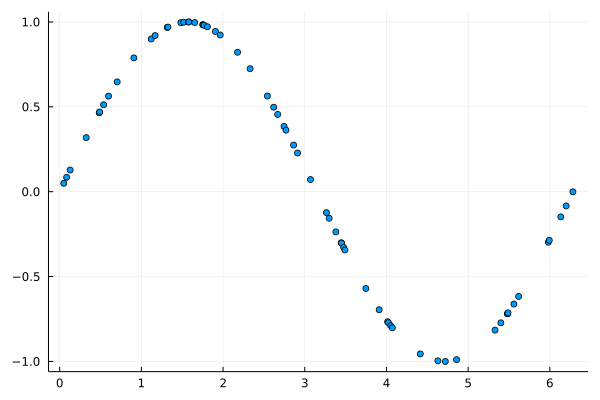
\includegraphics[width=0.8\textwidth]{images/nu_points.png}
    \caption{Non uniform sample points}
    \label{fig:nu_points}
\end{figure}

Using these samples, we can fit a simple piece-wise linear interpolation to sample uniform points as seem in Figure~\ref{fig:images-interp-png}.

\begin{figure}[htpb]
    \centering
    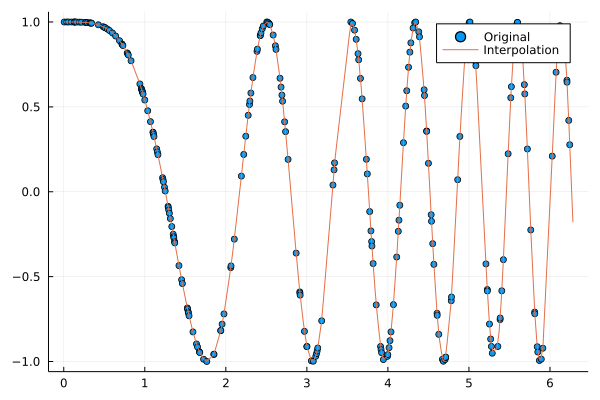
\includegraphics[width=0.8\textwidth]{images/interp.png}
    \caption{Piece-wise linear interpolant of nonuniform points}
    \label{fig:images-interp-png}
\end{figure}

In comparison, we can smooth the nonuniform points using the exponential of semicircle kernel as described in the previous section.
This convolution results in uniform samples as seen in Figure~\ref{fig:images-es-png}.

\begin{figure}[htpb]
    \centering
    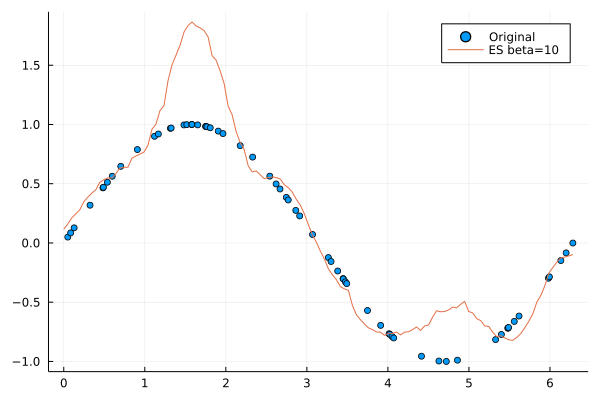
\includegraphics[width=0.8\textwidth]{images/es.png}
    \caption{Exponential of semicircle convolution of nonuniform sample points}
    \label{fig:images-es-png}
\end{figure}

Once resampled to uniform points, we can use the FFT to examine the Fourier spectrum of our samples.

\begin{figure}[htpb]
    \centering
    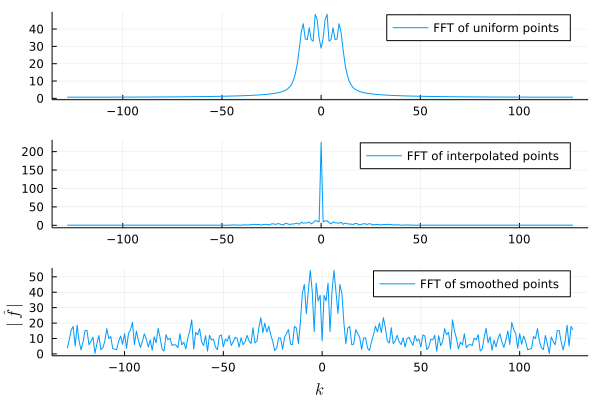
\includegraphics[width=0.8\textwidth]{images/fft_comparison.png}
    \caption{Comparison of spectra for uniform fft, interpolated fft, and smoothed nufft}
    \label{fig:images-fft-png}
\end{figure}

As expected, we can observe the reduction in accuracy using smoothing kernels as compared to the polynomial interpolation.
However, we can also quickly see the reduction in computational cost between the methods.
Figure~\ref{fig:images-speed-png} shows the speed of the approaches as a function of the number of nonuniform samples.

\begin{figure}[htpb]
    \centering
    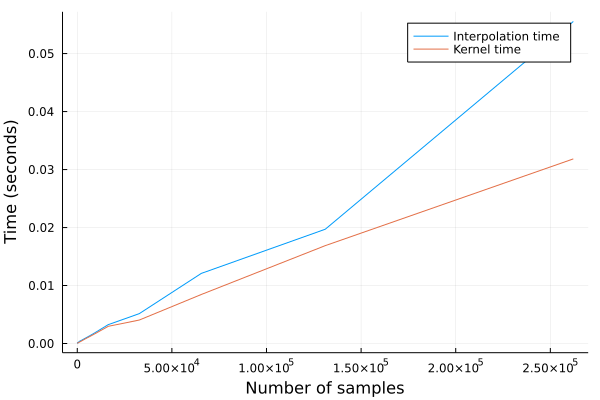
\includegraphics[width=0.8\textwidth]{images/speed.png}
    \caption{Comparison of method speed between interpolating and kernel methods}
    \label{fig:images-speed-png}
\end{figure}

The work presented in~\cite{IEEE-2021-Barnett} presents the exponential of semicircle kernel as an optimal balance between speed and accuracy, however it was difficult for us to choose the parameters in such as way as to obtain that accuracy.
%\section{Conclusion}

In conclusion, the nonuniform FFT is a particularly appealing tool in the fields of image and signal processing.
However, identifying a fast and accurate method has been a significant challenge for more than half a century.
Kernel methods which smooth delta spikes of nonuniform information have emerged as the favorite method of which we explored the Gaussian, Kaiser-Bessel, and exponential of semicircle versions.
These each present unique levels of smooth decay in real and Fourier space which affects the accuracy and speed of the resulting transformation.
Additionally, we explored a low-rank DFT version which relies on snapping nonuniform points to uniform points via Chebyshev polynomials.
Finally, we presented some simple numerical experiments comparing the exponential of semicircle smoothing kernel against the traditional interpolation then FFT procedure.
In general, this area is still being actively researched, and we were able to recognize the challenge of balancing speed and accuracy.

\bibliographystyle{unsrt}
\bibliography{reference}

\end{document}
